    \documentclass[times, utf8, diplomski, numeric]{fer}
\usepackage{booktabs}

\usepackage{pdfpages}
\usepackage{subcaption}
\usepackage{listings}
\usepackage[toc,page]{appendix}

\graphicspath{ {images/} }

\newcommand{\eng}[1]{(engl. \textit{#1})}

\begin{document}

\thesisnumber{1385}

\title{Implementacija kontinuirane isporuke programske podrške za operacijski sustav iOS}

\author{Ivan Rep}

\maketitle

% Ispis stranice s napomenom o umetanju izvornika rada. Uklonite naredbu \izvornik ako želite izbaciti tu stranicu.
\izvornik

% Dodavanje zahvale ili prazne stranice. Ako ne želite dodati zahvalu, naredbu ostavite radi prazne stranice.
\zahvala{}

\tableofcontents

\chapter{Uvod}
Uvod rada. Nakon uvoda dolaze poglavlja u kojima se obrađuje tema.

\chapter{Kontinuirana integracija}
Kontinuirana integracija je praksa spajanja svih razvojnih kopija koda s glavnom kopijom nekoliko puta dnevno. Termin je prvi predložio i iskoristio Grady Booch 1991. godine tijekom opisa metode danas poznate kao Boochova metoda \eng{Booch method}\citep{wiki:BoochMethod}.

Glavni cilj ove metode je smanjivanje broja konflikata prilikom spajanja različitih verzija koda. Tijekom razvoja programeri preuzimaju zajedničku \eng{master} kopiju izvornog koda \eng{source code} te nad njom obavljaju promjene. Lokalnu kopiju izvornog koda nazivamo razvojnom kopijom izvornog koda. Svaki programer ima vlastitu razvojnu kopiju izvornog koda.

Nakon implementacije željene promjene programer vlastitu razvojnu kopiju spaja s izvornom kopijom. Ovaj postupak nazivamo integracija izvornog koda. Ako zajednička kopija izvornog koda nije bila mijenjana od kako ju je programer preuzeo onda je moguće na nju jednostavno dodati promjene razvojne kopije. Međutim, ako je zajednička kopija izvornog koda mijenjana onda je potrebno na neki način spojiti promjene. Čim je duže programerova kopija izdvojena to je veća vjerojatnost promjene izvorne kopije. Što se kopije više razlikuju to je teže obaviti njihovo spajanje. Dodatno, spajanje često nije moguće obaviti automatski. Ova se pojava naziva konflikt te se javlja prilikom spajanja kopija koje su istovremeno modificirale isti dio izvornog koda. Programer u takvom slučaju prije integracije prvo mora preuzeti glavnu kopiju, ručno otkloniti konflikte koje prouzrokuje njegove promjene, te tada obaviti integraciju.

Nakon nekog vremena kopije mogu postati toliko različite da je vrijeme potrebno za njihovo spajanje duže od vremena koje je uloženo za implementaciju promjena. Ovaj se problem tada naziva \textit{pakao integracije}. Iako se ova situacija čini teško mogućom timovi mogu biti veliki, pritisak može biti visok i tempo naporan. Bez specificiranja postupka verzioniranja te automatizacije izgradnje i provjere ispravnosti projekti lako mogu završiti upravo u navedenom stanju.

Danas je kontinuirana integracija standardna praksa u razvoju programske potpore. Međutim, ona se značajno razlikuje od prakse koju je 1991. godine predložio Grady Booch. Danas se uz kontinuiranu integraciju usko vežu procesi automatizacije izgradnje, testiranja i osiguranja kvalitete programske potpore. Ovi pojmovi su postali toliko standardan dio kontinuirane integracije da mnogi upravo njih nazivaju kontinuiranom integracijom. Drugim riječima, pojam kontinuirane integracije danas podrazumijeva barem neku razinu automatizacije izgradnje i testiranje. S druge strane, učestalom spajanju radnih kopija se daje malo pozornosti. 

Odlomci ovog poglavlja proučavaju pojedini dio kontinuirane integracije: verzioniranje, izgradnju, testiranje i osiguranje kvalitete. Odlomak verzioniranje definira proces verzioniranja, sustave za kontrolu verzija te moderne procese verzioniranja koda. Dodatno, odlomak stavlja naglasak na usklađivanje procesa verzioniranja s temeljnom idejom kontinuirane integracije. Uz pregled procesa automatizacije izgradnje, testiranja i osiguranja kvalitete, navedeni odlomci definiraju i specificiraju razloge postojanja funkcionalnosti koje su realizirane u praktičnom dijelu rada.

Zadnji odlomak poglavlja prikazuje proces implementacije navedenih funkcionalnosti korištenjem alata Xcode Server.

\section{Verzioniranje}

Kao što je navedeno u prošlom odlomku, integracija je proces spajanja dviju različitih kopija izvornog koda. Međutim, nije definiran način kreiranja kopija, nit način njihovog održavanja i dijeljena među timom. Navedene zadaće obavlja sustav za verzioniranja.

Prvi dio odlomka daje pregled verzioniranja i sustava za verzioniranje. U nastavku su  definirane i analizirane prakse verzioniranja koje se koriste kod razvoja programske potpore. Prikazane su prednosti i mane svake prakse verzioniranja uz posebnu pozornost na učestalost obavljanja integracije. Na kraju odlomka je specificirana praksa verzioniranja koja se koristi u praktičnom dijelu ovog rada.

Verzioniranje je proces dodjele jedinstvenog imena ili jedinstvenog broja jedinstvenom stanju programske potpore\citep{wiki:SoftwareVersioning}. Identifikator omogućava jedinstvenu identifikaciju pojedinog stanja programske potpore te omogućava logičku organizaciju stanja.

U razvoju programske potpore se najčešće koriste dvije različite sheme verzioniranja. Unutarnje, inkrementalno verzioniranje koje se osvježava i nekoliko puta dnevno te vanjsko verzioniranje koje obilježava specifičnu verziju koda, na primjer verziju koda spremnu za objavu. Kod unutarnjeg verzioniranja sam identifikator nije bitan dokle god je on jedinstven. S druge strane, kako vanjsko verzioniranje nosi neko značenje, proces dodjele identifikatora je puno složeniji i ovisi o svrsi koje se pokušava postići.

Unutarnje verzioniranje koda se naziva kontrola verzija\citep{wiki:VersionControl}. Sustavi koji implementiraju proces kontrole verzija se nazivaju sustavi za kontrolu verzija. Najčešće su to samostalne aplikacije ali mogu biti i ugrađene u druge sisteme kao što su uređivači teksta, sustavi za kontrolu sadržaja i drugo.

Kroz povijest je razvijen veliki broj sustava za kontrolu verzija te je danas timski razvoj programske potpore ne zamisliv bez korištenja jednog od ovih alata.

\subsection{Sustavi za kontrolu verzija}

Danas se u praksi koriste dva alata: Apach Subversion i git. Apache Subversion, poznat i pod skraćenicom svn, je kreiran 2000. godine u sklopu projekta Apache Software Foundation zajednice. Alat je otvorenog koda, centraliziran, siguran i jednostavan za korištenje. Obično postoji jedan glavni repozitorij kojeg programeri kloniraju, uređuju te ga zatim sinkroniziraju s glavnim repozitorijem.

Git je kreirao Linus Torvalds 2005. godine zbog nezadovoljstva tadašnjim sustavima za kontrolu verzija. Izdan je kao alat otvorenog koda te je ubrzo okupio veliku podršku u zajednici. Za razliku od svna, git je distribuirani sustav. Isti repozitoriji mogu postojati na proizvoljnom broju uređaja u proizvoljnom broju stanja. Navedeni se repozitoriji mogu klonirati, usklađivati i uređivati neovisno jedan od drugom. Zbog navedenog je pomoću gita moguće implementirati proizvoljan proces verzioniranja. Bio to centralizirani repozitorij nalik na svnov pristup, pristup s osobama zaduženim za odobravanje promjena, distribuirani model i drugi. Najvažnije, git je jednostavan ali vrlo moćan alat. Lako je implementirati osnovne funkcionalnosti dok istovremeno postoji podrška za vrlo kompleksne pothvate.

Svn je stariji sustav međutim još je uvijek široko korišten u velikom broju kompanija i projekata otvorenog koda. Međutim, git je značajno dobio na popularnosti u zadnjem desetljeću. Njegova jednostavnost i podržanost ga čine lakšim za upoznavanje i korištenje. Danas git preuzima tržište te ga koristi velika većina novih projekata. U ostatku ovog rada ću koristiti git. Sve se funkcionalnosti mogu, uz manju modifikaciju, implementirati i u svnu.

\subsection{Uvod u git}

Temeljne funkcionalnosti git alata su repozitoriji i grane. Repozitorij je direktorij koji je verzioniran korištenjem git sustava za kontrolu verzija. Ovaj repozitorij sadrži direktorij “.git” koji specificira na koji se način verzionira repozitori te sadrži informacije o repozitoriju.

Repozitoriji se mogu klonirati na istom ili drugom uređaju. Klonirani repozitorij je novi repozitorij koji sadržava svu povijest kloniranog repozitorija. Promjene koje se obavljaju u kloniranom repozitoriju nemaju nikakvog utjecaja na izvorni repozitorij. Međutim, promjene obavljene u kloniranom repozitoriju se mogu, uz postojanje odgovarajuće autorizacije, prenijeti na izvorni repozitorij. Prijenos promjena se ne mora obavljati isključivo između izvornog i kloniranog repozitorija, već se može obaviti između bilo koja dva povezana repozitorija.

\begin{figure}
    \centering
    \begin{minipage}{.5\textwidth}
        \centering
        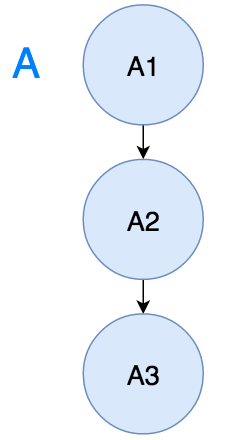
\includegraphics[scale=0.6]{Initial_commit}
        \caption{Grana s tri potvrde}
        \label{fig:Initial_commit}
    \end{minipage}%
    \begin{minipage}{.5\textwidth}
        \centering
        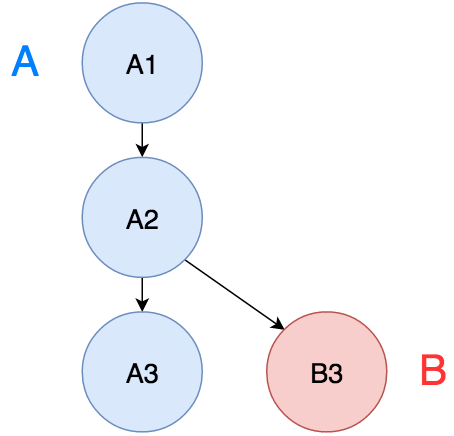
\includegraphics[scale=0.6]{Branching}
        \caption{Grananje}
        \label{fig:Branching}
    \end{minipage}
\end{figure}

\begin{figure}[b!]
    \centering
    \begin{subfigure}{.49\textwidth}
        \centering
        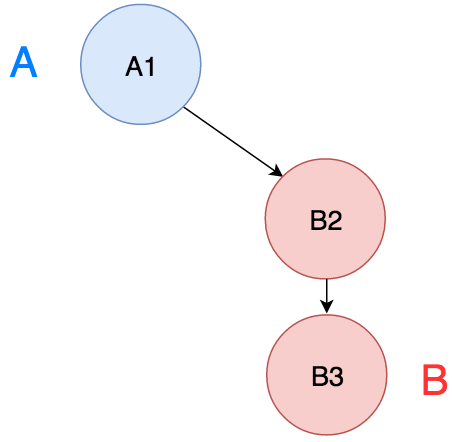
\includegraphics[scale=0.6]{FastForwardA}
        \caption{Stanje prije spajanja}
        \label{fig:FastForwardA}
    \end{subfigure}
    \begin{subfigure}{.49\textwidth}
        \centering
        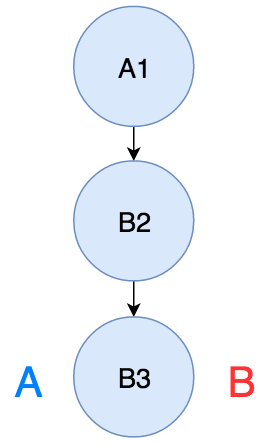
\includegraphics[scale=0.6]{FastForwardB}
        \caption{Stanje nakon spajanja}
        \label{fig:FastForwardB}
    \end{subfigure}
    \caption{Spajanja dodavanje promjena}
    \label{fig:FastForward}
\end{figure}

Prilikom kreiranja git repozitorija stvara se i glavna grana (eng. master branch) repozitorija. Grana je definirana slijedom promjena koje su primijenjene na njoj. Modificiranje dokumenata u repozitorija ne uzrokuje samo po sebi stvaranje nove verzije. Obavljene modifikacije je potrebno potvrditi \eng{commit}. Potvrđivanje modifikacija kreira novu verziju izvornog koda na trenutnoj grani te osvježava njeno stanje. Potvrđivanje promjena je prikazano na slici \ref{fig:Initial_commit}. Repozitorij koda se stvara kreiranjem glavne grane i obavljanjem inicijalnog potvrđivanja \eng{initial commit}. Glavna grana je označena slovom A. Inicijalno potvrđivanje je označeno s A1, dok su naknadna potvrđivanja označena s A2 i A3.

Nova grana se može kreirati iz bilo kojeg stanja postojeće granje. Ovaj se postupak naziva grananje \eng{branching}. Izvorna i klonirana grana dijele zajedničku povijest do trenutka grananja. Daljnje promjene se primjenjuju samo na izvornu ili kloniranu granu. Slika \ref{fig:Branching} prikazuje postupak grananja. Grana B se kreira iz stanja A2 grane A. Grane A i B dijele dva zajednička stanja A1 i A2. Ova stanja nazivamo zajednička povijest grana. Nakon grananja na granu B dodajemo dva nova stanja B2 i B3.


\begin{figure}[b!]
    \centering
    \begin{subfigure}{.49\textwidth}
        \centering
        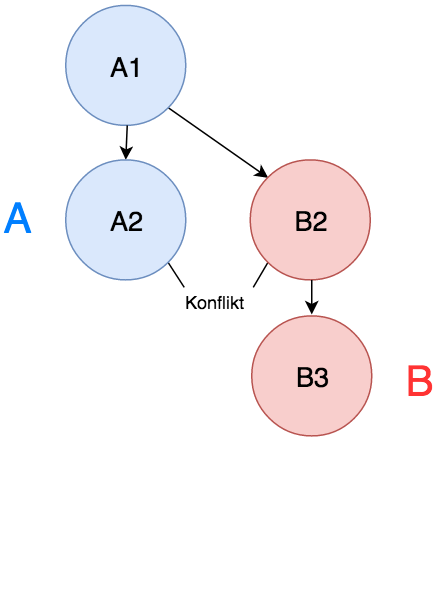
\includegraphics[scale=0.6]{ConflictA}
        \caption{Stanje prije spajanja}
        \label{fig:ConflictA}
    \end{subfigure}
    \begin{subfigure}{.49\textwidth}
        \centering
        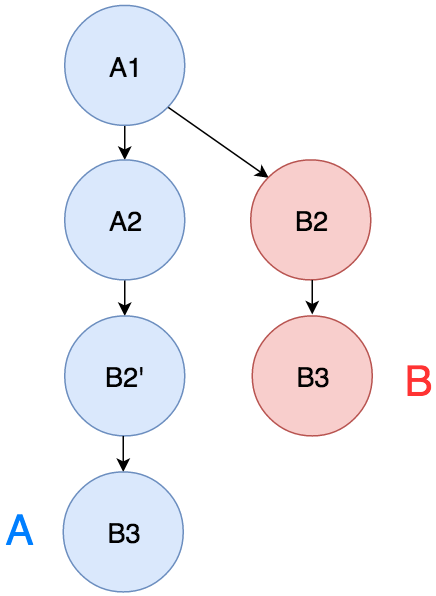
\includegraphics[scale=0.6]{ConflictB}
        \caption{Stanje nakon spajanja}
        \label{fig:ConflictB}
    \end{subfigure}
    \caption{Spajanja otklananjem konflikta}
    \label{fig:Conflict}
\end{figure}

Grane je također moguće spojiti. Spajanje grana dodaje promjene obavljene na izvornoj \eng{source} grani u odredišnu \eng{destionation} granu. Spajanje je moguće obaviti na nekoliko načina ovisno o odnosu dviju grana koje se spajaju. Slika \ref{fig:FastForward} prikazuje najjednostavniji odnos dviju grana kod spajanja. Nakon grananja grane B iz stanja A2 grane A na granu B se dodaju dva nova stanja, B2 i B3. U međuvremenu je grana A ostala nepromijenjena. Zbog navedenog je spajanje grana moguće obaviti jednostavno dodavanjem promjena B grane na vrh A grane, \eng{fast forward}. Slike \ref{fig:FastForwardA} prikazuje stanje prije spajanja dok slika \ref{fig:FastForwardB} prikazuje stanje nakon spajanja. Dodatno, samo spajanje je moguće označiti dodavanjem dodatnog stanja na granu na kojoj se obavlja spajanje.

Postupak se komplicira ako je odredišna grana modificirana nakon grananja. U navedenom slučaju nije moguće promjene obavljene u izvorišnoj gani samo dodati na vrh odredišne grane, nego je promjene potrebno spojiti. Proces spajanja ovisi o tome postoje li konflikti između promjena. Ako ne postoji, spajanje je moguće obaviti jednako kao na slici \ref{fig:FastForward}, jednostavno dodavanjem promjena na vrh odredišne grane.

Međutim, ako promjene izazivaju konflikte, onda je te konflikte potrebno ručno razriješiti. Otklanjanje konflikata uzrokuje izmjenom verzija jedne ili obje grane. Proces otklanjanja konflikata se najčešće odrađuje dodavanjem jedne po jedne verzije izvorne grane na odredišnu granu. Ako dodana verzija ne izaziva konflikt, ona se jednostavno dodaje na vrh odredišne grane. Međutim, ako verzija izaziva konflikt, tada se isti otklanja modificirajući dodanu verziju. Slika \ref{fig:Conflict} prikazuje proces spajanja grana s konfliktom. Konflikt je nastao između verzija A2 i B2. Konflikt se otklanja dodavanjem verzije B2 na vrh A grane i njenim modificiranjem. Ovo je stanje označeno s B2'. Stanje B3 ne izaziva konflikt te se samo dodaje na vrh A grane. Rezultat spajanja su dvije grane A i B različitih povijesti.

\begin{figure}[h!]
    \centering
    \begin{subfigure}{.3\textwidth}
        \centering
        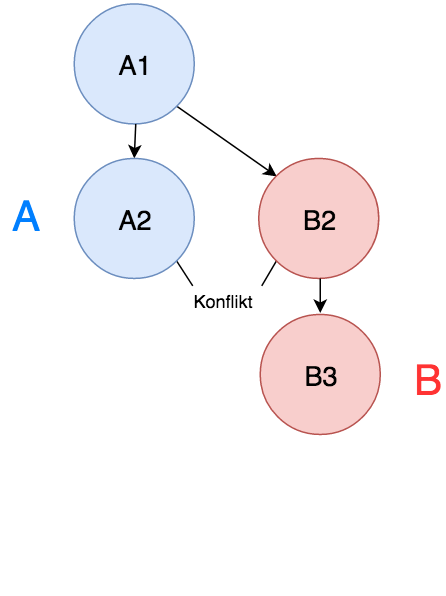
\includegraphics[scale=0.5]{RebaseA}
        \caption{Početno stanje}
        \label{fig:RebaseA}
    \end{subfigure}
    \begin{subfigure}{.3\textwidth}
        \centering
        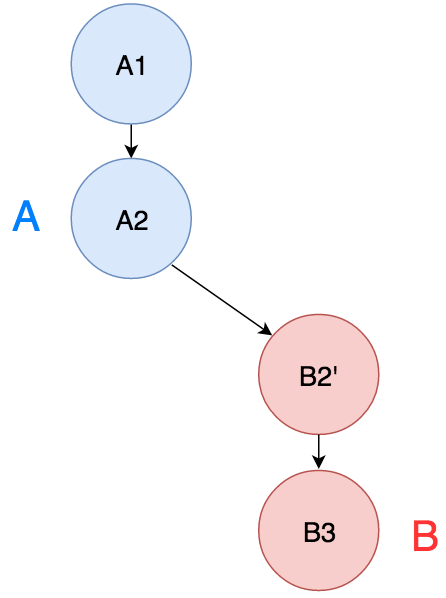
\includegraphics[scale=0.5]{RebaseB}
        \caption{Stanje nakon \textit{rebase}}
        \label{fig:RebaseB}
    \end{subfigure}
        \begin{subfigure}{.3\textwidth}
        \centering
        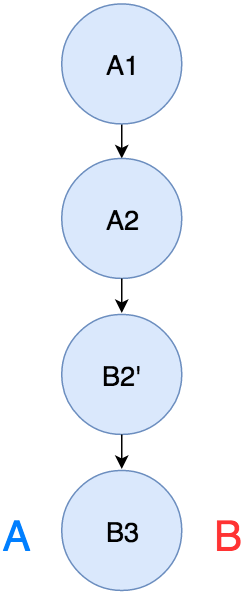
\includegraphics[scale=0.5]{RebaseC}
        \caption{Stanje nakon spajanja}
        \label{fig:RebaseC}
    \end{subfigure}
    \caption{Spajanje \textit{rebase} postupkom}
    \label{fig:Rebase}
\end{figure}

Gore naveden slučaj se često rješava postupkom pod nazivom \textit{rebase}. Postupak prije spajanja u povijest izvorišne grane dodaje sve verzije nastala u odredišnoj grani nakon grananja. Verzije se dodaju odmah nakon stare točke grananja čime se točka grananja pomiče na zadnju verziju A grane. Slika \ref{fig:RebaseB} prikazuje stanje nakon obavljanja \textit{rebase} postupka na grani B. Sada su grane u stanju jednakom onom na slici \ref{fig:FastForward} te je spajanje moguće obaviti dodavanjem promjena na vrh odredišne grane. Stanje B2 se još uvijek mijenja, međutim sada je povijest repozitorija linearna.

\subsection{Implementacije procesa verzioniranja}

Proces verzioniranja je moguće implementirati na nekoliko različitih načina. Programer koji samostalno radi na projektu najčešće koristi repozitorij s jednom granom na kojoj obavlja promjene i proizvoljno sinkronizira lokalni s glavnim repozitorijem. Međutim, ovaj pristup je vrlo teško održiv u timskom radu. Učestalo preplitanje različitih tokova razvoja na jednoj grani značajno otežava praćenje promjena i čini gotovo nemogućim vraćanjem promjena unazad.

Danas se u praksi koristi nekoliko različitih procesa verzioniranja \eng{versionining workflows}. Ovaj odlomak obrađuje centralizirani proces \eng{centralized workflow}, proces grananja funkcionalnosti \eng{feature branch workflow}, \textit{gitflow} proces \eng{gitflow workflow} i proces forkanja \eng{forking workflow}. Svaki od navedenih pristupa ima svoje prednosti i mane te se koristi u različitim tipovima projekta\citep{versioningWorkflows}.

Centralizirani proces koristi jedan glavni i više lokalnih repozitorija. Najčešće se koristi samo jedna, glavna grana. Svaki programer kreira lokalnu kopiju glavnog repozitorija na kojoj obavlja promjene. Nakon obavljanja željenih promjena iste spaja s glavnom granom centralnog repozitorija. Na pojedinom je programeru da vlastitu, lokalnu verziju repozitorija drži usklađenom s glavnim repozitorijem. Glavni repozitorij predstavlja službeno stanje projekta zbog čega treba posebnu pažnju obratiti na održavanje njegove povijesti. Izmjena povijesti glavnog repozitorija može dovesti lokalne repozitorije u nekonzistentno stanje zbog čega se ona smatra vrlo lošom praksom. Zbog navedenog, ako lokalna kopija izaziva konflikt pri spajanju, konflikt je potrebno otkloniti na lokalnoj kopiji te promjene zatim spojiti s centralnim repozitorijem. Centralizirani proces je vrlo jednostavan te je sličan načinu rada svna.

\begin{figure}[b]
    \centering
    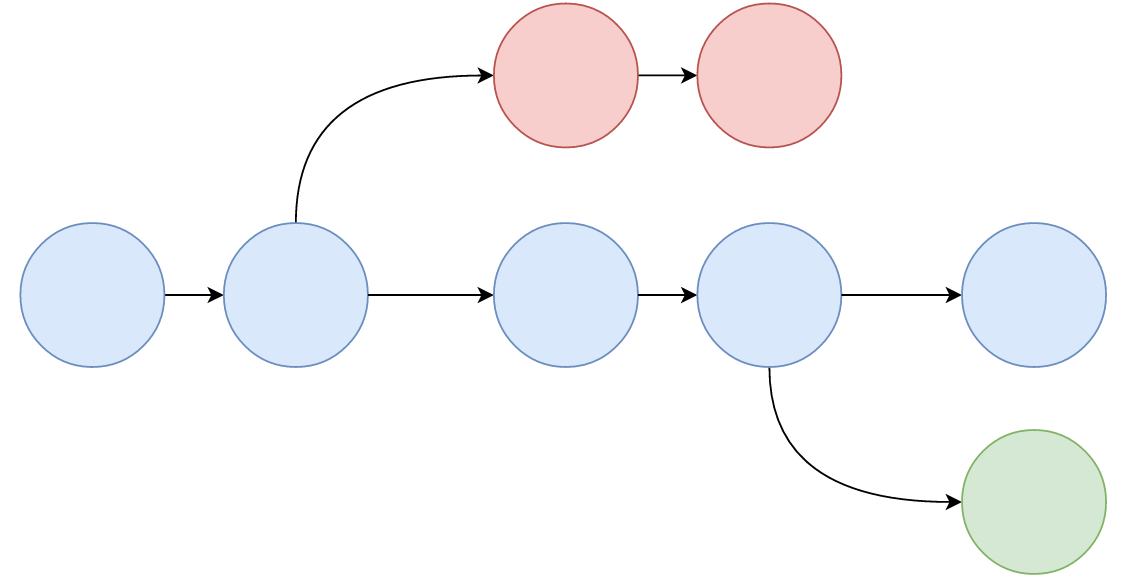
\includegraphics[scale=0.5]{FeatureBranch}
    \caption{Primjer proces grananja funkcionalnosti}
    \label{fig:FeatureBranch}
\end{figure}

Proces grananja funkcionalnosti nastoji otkloniti glavni nedostatak centraliziranog procesa, učestalo preplitanje različitih tokova razvoja. Proces grananja funkcionalnosti također ima jedan glavni i više lokalnih repozitorija. Razlika je u tome što se funkcionalnost implementira u grani kreiranoj specifično za nju. Programer za novu funkcionalnost kreira novu granu u lokalnom repozitoriju te u nju dodaje promjene. Po završetku implementacije funkcionalnosti programer granu spaja s glavnom granom centralnog repozitorija. Ovaj proces daje jasniji uvid u napredak projekta i implementirane funkcionalnosti. Dodatno, proces timu daje priliku revizije obavljenih promjena. Umjesto direktnog spajanja grane moguće je kreirati zahtjev za spajanjem \eng{merge request}. Zahtjev za spajanjem dodatno opisuje promjene ostvarene u sklopu grane te timu daje priliku za komunikaciju i reviziju obavljenih promjena.

Gitflow proces također koristi jedan centralni i više lokalnih repozitorija. Za razliku od prijašnja dva procesa, gitflow proces povijest repozitorija prati kroz glavnu i razvojnu granu. Razvojna grana \eng{develop branch} je vrlo slična glavnoj grani u procesu grananja funkcionalnosti. Grana za novu funkcionalnost se kreira iz razvojne grane te se po završetku implementacije u nju spaja. S druge strane, glavna grana sadrži samo produkcijske verzije izvornog koda, odnosno one verzije projekta koje su obavljene korisniku. Kad tim odluči objaviti novu verziju projekta, kreira se nova grana iz trenutnog stanja razvojne grane. Nakon završetka provjere ispravnosti grana se spaja s glavnom, i po potrebi razvojnom granom. Nova verzija glavne grane se zatim objavljuje. Verzije na glavnoj grani se označavaju sa objavljenom verzijom projekta.

Primjer korištenja gitflow procesa je prikazan na slici \ref{fig:Gitflow}. Crvenom bojom je prikazana glavna grana a plavom razvoja grana. Grane funkcionalnosti, prikazane zelenom i žutom bojom se granaju iz razvojne grane te u nju spajaju. Bijelom bojom je označena grana pripreme za objavu nove verzije projekta. Nakon obavljanja pripreme za objavu grana se spaja s glavnom granom tima kreirajući novu produkcijsku verziju, te s razvojnom granom kako bi promjene nastale kod pripreme za objavu bile dodane projektu.

\begin{figure}
    \centering
    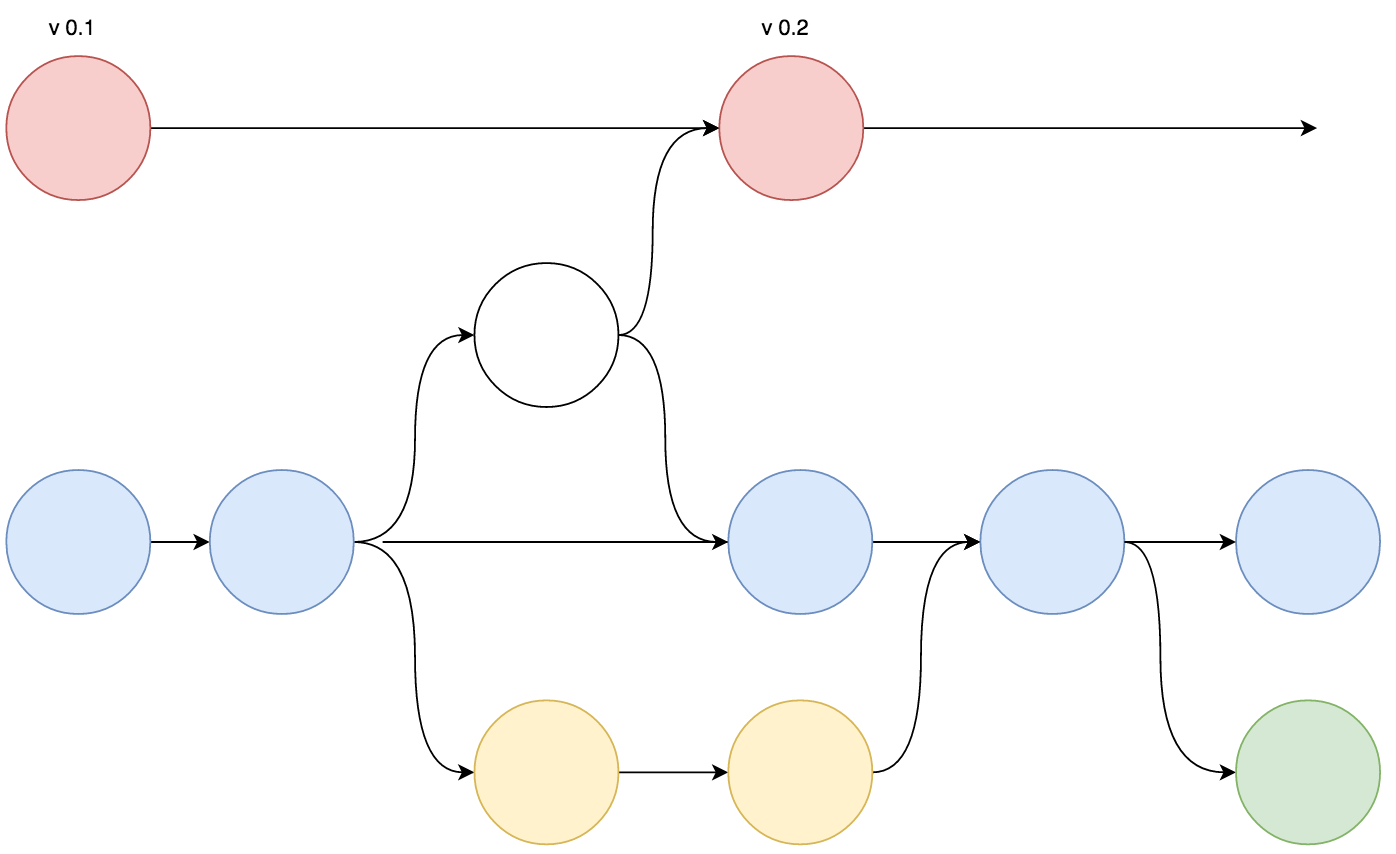
\includegraphics[scale=0.5]{Gitflow}
    \caption{Primjer gitflow procesa}
    \label{fig:Gitflow}
\end{figure}

Navedeni pristup olakšava upravljanje objavom projekta. Buduće da je krucijalno objaviti ispravan produkt sam proces objave treba biti kontroliran i a produkt temeljito testiran. Izdvajajući proces objave na glavnu granu omogućava istovremeno testiranje produkcijske verzije i nastavak rada na novim funkcionalnostima.

Za razliku od ostalih procesa promatranih u ovom poglavlju, forking proces nema centralni repozitorij već svaki sudionik ima vlastiti javni i privatni repozitorij. Programer vlastiti javni repozitorij kreira kopiranjem nekog drugog javnog repozitorija. Zatim iz vlastitog javnog repozitorija kreira vlastiti privatni repozitorij. Promjene obavlja na privatnom repozitoriju te ih proizvoljno spaja s javnim repozitorijem. Navedene promjene zatim može iskoristiti netko drugi kloniranjem repozitorija ili spajanjem promjena s postojećim repozitorijem. Dodatno, programer može predložiti dodavanje promjena nekom drugom repozitoriju. Navedeni se proces naziva zahtjev za povlačenjem \eng{pull request}.

Forking proces se najčešće primjenjuje za projekte otvorenog koda. On omogućuje svakom članu zajednice kloniranje, modifikaciju i objavu promjena obavljenih na projektu. Dodatno, zahtjev za spajanje daje vrlo dobar uvid u obavljene promjene bez modifikacije izvornog repozitorija.

\subsection{Kontinuirana integracija i verzioniranje}

Osnova kontinuirane integracije je kontinuirano, odnosno učestalo spajanje radnih kopija s glavnom kopijom. Kad bi se vodili samo ovim principom centralizirani repozitorij bi najbolje zadovoljavoao naše zahtjeve. Međutim, centralizirani repozitorij se danas korisiti gotovo isključito za privatne ili vrlo jednostavne projekte.

Drugi procesi rjeđe obavljaju integraciju radnih kopija. Na primjer, gitflow proces integraciju radne kopije s glavnom kopijom obavlja po završetku implementacije funkcionalnosti. Što je veća funkcionalnost koja se implementira, to će duže radna kopija ostati izdvojena. Zbog navedenog je potrebno posao razdijeliti na male dijelove. Navedeno ne pridonosi samo procesu kontinuirane integracije, već olakšava praćenje projekta te je sastavni dio agilnog pristupa razvoja programske potpore. Prednosti koje napredniji pristupi verzioniranju pruža, kao što su lakše praćenje razvoja, zahtjevi za spajanjem i lakše objave projekta u produkciju nadilaze nešto duže vrijeme izdvojenosti radnih kopija.

U praktičnom dijelu ovog projekta koristim gitflow proces. Ovaj proces najbolje odgovara zahtjevima i tipu projekta. Dodatno, gitflow proces omogućava jednostavniju implementaciju kontinuirane dostave i isporuke. Uz glavnu i radnu granu, repozitoriju ću po potrebi dodavati dodatne grane. Na primjer, isporuku verzija programske potpore za testiranje ću izdvojiti u zasebnu granu. Ovo omogućava lako praćenje testnih verzija te olakšava implementaciju procesa isporuke testne verzije.

Proces kontinuirane integracije će se obavljati na svim granama. Dodatno, spajanje bilo koje dvije grane neće biti moguće ako rezultat spajanja ne prolazi sve kriterije kontinuirane integracije.


\section{Automatizacija izgradnje}

Povijesno, pojam izgradnja se često koristio kao sinonim pojma kompajliranje. Kompajliranje \eng{compilation} je proces prevođenja koda iz jednog jezika u drugi uz očuvanje izvorne funkcionalnosti. Kod se u ovom procesu često dodatno optimizira. Najčešći razlog kompajliranja je prevođenje koda u jezik kojeg može razumjeti i time izvršiti procesor. Rezultat kompajliranja je izvršni program, odnosno program koji se može izvršiti. Kompajliranje je složena funkcija koja se najčešće obavlja u više prolaza. Jezici koji se kompajliraju se nazivaju kompajlirani jezici \eng{compiled languages}.

Interpretirani jezici \eng{interpreted languages} se ne prevode već interpretiraju. Oni se izvršavaju na pomoćnom programu naziva interpreter koji uzima naredbe izvornog jezika te ih prevodi u naredbe koje računalo razumije. Danas gotovo niti jedan jezik nije u cijelosti kompajliran ili interpretiran već koristi kombinaciju obje metode s ciljem optimizacije performansi.

\begin{figure}
    \centering
    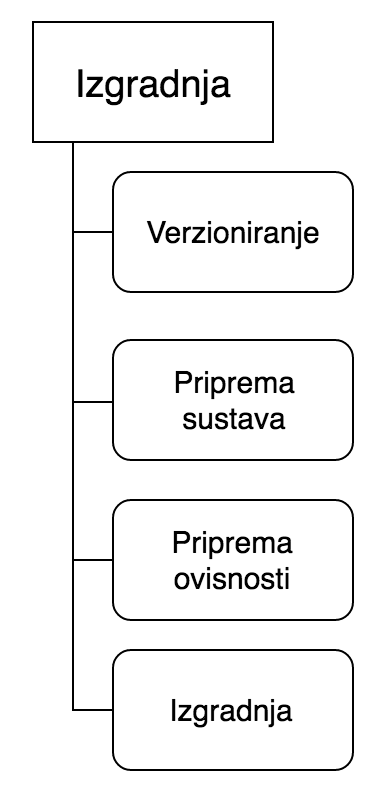
\includegraphics[scale=0.5]{BuildProcess}
    \caption{Generalna podjela procesa izgradnje}
    \label{fig:BuildProcess}
\end{figure}

Danas s pojmom izgradnje vežemo sve procese koji su dio pretvaranja izvornog koda u artefakt koji možemo koristiti. Ovisno o jeziku i alatima koje koristimo, proces izgradnje može značajno oscilirati u svojoj veličini. Generalno proces izgradnje možemo podijeliti na verzioniranje, pripremu sustava za izgradnju, dohvat i pripremu ovisnosti \eng{dependancies} te kompajliranje. Verzioniranjem odabiremo željenu verziju izvornog koda koju koristimo za izgradnju artefakta. Priprema za izgradnju dovodi računalo u stanje potrebno za obavljanje izgradnje. Izvorni kod često sadržava upute za pripremu sustava kao što su potrebni alati, verzije alata i konfiguraciju projekta. Dohvat i priprema ovisnosti osigurava postojanje ispravnih ovisnosti korištenih u izvornom kodu. Ovisnosti dijelimo na dva tipa, službene ovisnosti koje smatramo dijelom razvojne okoline i vanjske \eng{third party} ovisnosti, najčešće razvijene od strane zajednice. Kompajliranje prevodi izvorni kod u izvršivi artefakt. Kod interpretiranih jezika ovaj je proces često zamijenjen statičkom i dinamičkom provjere izvedivosti programa. Proces izgradnje je prikazan na slici \ref{fig:BuildProcess}.

Izgradnje provjerava je li zadana verzija izvornog koda izgradiva. Kod je izgradiv ako se u procesu izgradnje ne desi pogreška, odnosno ako se isti ispravno izvrši. Pogrešku može izazvati neispravnost u izvornom, neispravna konfiguracija sustava, nepostojanje potrebnog alata ili neki drugi nedostatak. Izgradivost sustava je preduvjet za  testiranja i isporuku. Samim time je automatizacija izgradnje preduvjet za automatizaciju testiranja i automatizaciju isporuke.

Proces verzioniranja je definiran u prošlom odlomku. Proces pripreme sustava se uglavnom sastoji od dohvata potrebnih alata te je definiran gdje je to potrebno. Dohvat ovisnosti i izgradnja je detaljnije specificirana u nastavku. Primjeri izvedbe cijelog procesa izgradnje je prikazan u dodatku A.

\subsection{Upravljanje ovisnostima}

Prije izgradnje projekta je potrebno dohvatiti sve ovisnosti i alate koje projekt zahtjeva. Alat xcodebuild, kojeg koristimo za izgradnju programske potpore za iOS operacijske sustave, sadrži sve službene biblioteke i alate potrebne za izgradnju. Međutim, ako projekt koristi vanjske biblioteke iste je potrebno dohvatiti i pripremiti za korištenje. Za dohvaćanje vanjskih biblioteka se u iOS razvoju koriste dva alata: \textit{CocoaPods} i \textit{Carthage}.

CocoaPods je vrlo jednostavan centralizirani sustav za upravljanje ovisnostima. Za dohvaćanje ovisnosti je potrebno samo specificirati iste u datoteci imena \textit{Cartfile}. Alat samostalno kreira i konfigurira novo radno okruženje u koje dodaje osnovni projekt i sve ovisnosti. Jedino što programer mora napraviti je razvoj obavljati u radnom okruženju a ne u osnovnom projektu.

Najveći problem alata je učestala modifikacija radnog okruženja i njegovih konfiguracija. Drugim riječima, alat mijena postavke izgranje što može uzrokovati neželjeno ponašanje. Dodatno, budući da je alat centraliziran, sve korištene biblioteke moraju biti registrirane u CocoaPods sustavu. Navedeno otežava korištenje privatnih biblioteka i biblioteka u razvoju.

Carthage je decentralizirani alat za upravljanje ovisnostima. Sustav omogućava jednostavno dohvaćanje i izgradnju biblioteke. Za razliku od CocoaPods alata, Carthage ne modificira radno okruženje. Navedeno znači da je ovisnost potrebno samostalno uključiti u projekt ali u istom trenutku otklanja neželjene posljedice koje nosi CocoaPods.

Oba sustava se široko koriste te izbor uvelike ovisi o osobnom ukusu. Zbog navedenog u radu koristim oba alata.

\subsection{Izgradnja}

Izgradnja iOS aplikacija se obavlja korištenjem alat \textit{xcodebuild}\citep{xcodebuild}. Alat je razvio Apple za izgradnju programske potpore za macOS operacijski sustav. Alat je vrlo moćan te pruža veliki broj funkcionalnosti i mogućih konfiguracija. Alat je proširen te danas podržava izgradnju aplikacija za iOS, tvOS i watchOS operacijske sustave. Alat izgradnju obavlja na temelju Xcode projekta. Prije definiranje procesa izgradnje se je potrebno upoznati s Xcode projektom.

Xcode je službeni Appleov alat za razvoj programske potpore za iOS i macOS operacijske sustave. Na tržištu postoji nekoliko alternativa ali je Xcode daleko najkorišteniji. Svi alati koriste xocdebuild za izgradnju te zbog toga imaju istu strukturu projekta. Ovaj tip projekta se naziva Xcode projekt.

Xcode projekt sadrži jedan ili više ciljeva \eng{target} i jednu ili više shema \eng{scheme}. Cilj definira resurse koji se koriste kod izgradnje te specificira postavke i rezultat procesa izgradnje. Jedan projekt može sadržavati više ciljeva. Više ciljeva se uglavnom koristi za različite distribucije istog projekta, na primjer za distribuciju aplikacija koje podržavaju različite verzije operacijskog sustava. Dodatno, budući da su svi Appleovi operacijski sustavi vrlo slični, isti projekt je pomoću više ciljeva moguće distribuirati za različite operacijske sustave. Shema definira koji se cilj koristi za koju operaciju. Projekt može implementirati više shema kako bi objedinio operacije za pojedinu distribuciju. Odnos cilja i sheme je prikazan na slici \ref{fig:TargetScheme}. Projekt sadrži tri cilja i dvije sheme. Sheme različito definiraju koji se cilj koristi za koju operaciju.

\begin{figure}
    \centering
    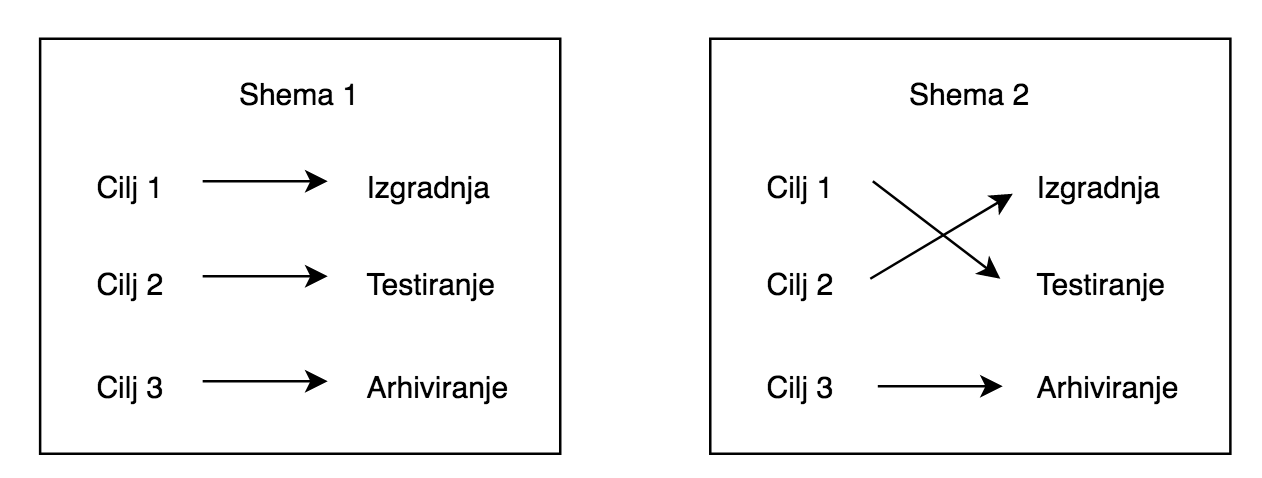
\includegraphics[scale=0.5]{TargetScheme}
    \caption{Xcode projekt s tri cilja i dvije sheme}
    \label{fig:TargetScheme}
\end{figure}

Xcode projekte je moguće grupirati u Xcode radno okruženje \eng{workspace}. Radno okruženje olakšava segmentiranje velikog projekta i olakšava upravljanje ovisnostima.

Alat xcodebuild uz izgradnju pruža i operacije kao što su testiranje, analiziranje, profiliranje i arhiviranje. Testiranje pokreće testni cilj i objavljuje njegove rezultate. Analiziranje prikuplja informacije o izvornom kodu dok profiliranje pruža veliki broj alata za praćenje ponašanja aplikacije u izvođenju. Arhiviranje služi za distribuiranje aplikacije. Ovaj postupak proizvodi arhivu koju je zatim moguće objaviti na AppStoreu ili ju instalirati direktno na uređaj.

Za pokretanje procesa izgradnje je dovoljno pozvati xcodebuild alat iz ljuske uz korištenje operacije za izgradnju. Proces ne rezultira izvršivim artefaktom već samo provjerava je li sustav izgradiv. Projekt koji je izgradiv je moguće pokrenuti na uređaju također korištenjem alata xcodebuild ili ga arhivirati. Arhiviranje rezultira prenosivim artefaktom koji je moguće objaviti na AppStoreu ili ga ručno instalirati na uređaj.

\subsection{Automatizacija izgradnje korištenjem Xcode Servera}

Automatizaciju izgradnje možemo ostvariti automatizacijom pozivanja alata xcodebuild pri svakoj novoj verziji na željenoj grani. Dovoljno je samo pozvati naredbu uz specificiranje projekta i cilja. Objava rezultata je nešto složenija. Trebali bi parsirati izlaz xcodebuild alata i formatirati ga tako da je lako čitljiv. Na sreću, postoji veliki broj alata koji cijeli ovaj proces već implementiraju.

U ovo radu koristim alat Xcode Server. Dodatak B objašnajva zašto sam od velikog broja alata odabrao upravo njega. Alat je zapravo spoj dva alata. Već spomenutom Xcodea i macOS Servera. Alat Xcode već koristimo te on ne predstavlja dodatno opterećenje. macOS Server je Appleov alat za obavljanje automatizacije. Alat je besplatan za osobe s Apple developer računom koji je potreban za razvoj iOS aplikacija.

Xcode Server je razvijen upravo za implementaciju kontinuirane integracije za Xcode projekte. Kao takav dolazi opremljen upravo funkcionalnostima koje želimo implementirati. Za automatizaciju cijelog gore navedenog procesa je potrebno samo odabrati nekoliko opcija unutar alata Xcode. Cijeli proces je prikazan u dodatku B.

Nakon instalacije macOS Servera alat je potrebno uskladiti s Xcode alatom koji koristimo u razvoju. U Xcodeu odabrati opciju \textit{Product -> Create bot}. Alat samostalno otkriva način verzioniranja i lokaciju repozitorija. Nakon autorizacije pristupa repozitoriju slijedi nekoliko prozora u kojima je moguće konfigurarati opcije kontinuirane integracije. Među ostalim, moguće je konfigurirati kada se izvršava integracija, koja shema i cilj se koristi, koje se operacije izvršavaju te dodati pozive skripti prije i poslje integracije.









\chapter{Zaključak}
Zaključak.

\bibliography{literatura}
\bibliographystyle{fer}

\begin{sazetak}
Sažetak na hrvatskom jeziku.

\kljucnerijeci{Ključne riječi, odvojene zarezima.}
\end{sazetak}

% TODO: Navedite naslov na engleskom jeziku.
\engtitle{Title}
\begin{abstract}
Abstract.

\keywords{Keywords.}
\end{abstract}




\begin{appendices}



\chapter{Ručna integracija i isporuka iOS aplikacija}

Ovaj dodatak je tehnički usmjeren pregled ručne implementacije procesa integracije i isporuke iOS aplikacije. Glavni cilj dodatka je upoznati se s alatima koje koristimo kod razvoja, integracije i isporuke iOS aplikacija. Sam postupak automatizacija donosi svoje prepreke, zbog čega je lakše prvo definirati postupak koji automatiziramo.

Prvi dio dodatka specificira alate koje koristim u razvoju, integraciji i isporuci te njihovu instalaciju i pripremu. Drugi dio obrađuje integraciju a treći isporuku.

Primjeri su napisani korištenjem operacijskog sustava \textit{macOS Sierra 10.12.4}.

\section{Alati}

Sve naredbe su definirane za \textit{bash} ljusku. Ovoj ljusci je najjednostavnije pristupiti korištenjem \textit{termianl} aplikacije dostupne na svakoj instalaciji macOS operacijskog sustava. Naravno, moguće je koristiti bilo koji drugi tekstualno sučelje s pristupom bash ljusci.

Za provjeru postojanja alata koristim sljedeći naredbu. Naredbu ću koristiti za provjeru postojanja alata i izbjegavanje nepotrebne reinstalacije.

\begin{verbatim}
if which {ime_naredbe} >/dev/null; then
    echo "{ime_naredbe} installed"
else
    echo "{ime_naredbe} not installed"
fi
\end{verbatim}

Za razvoj iOS aplikacija koristim alat Xcode. Na tržištu postoji nekoliko sličnih alata, ali je Xcode daleko najpopularniji te ga koristimo i za ostvarenje automatizacije integracije. Alat je moguće instalirati korištenjem App Store aplikacije. Za testiranje procesa koje ću implementirati u ostatku ovog dodatka kreiram jednostavan testni projekt. Projekt je iOS aplikacija imena \textit{Diplomski\_rad} te sadrži jednu shemu istog imena. Projekt sadrži tri cilja: iOS aplikaciju, \textit{unit} i \textit{ui} testove.

\textit{Hombrew} je alat za instaliranje i upravljanje alatima za macOS operacijski sustav. Alat olakšava instalaciju i konfiguraciju nekoliko alata koje koristimo u sklopu razvoja. Mana ovog alata je zahtijevanje \textit{sudo} pristupa zbog čega instalaciju alata nije moguće automatizirati.

Homebrew je moguće preuzeti korištenjem sljedeće naredbe. Naredba prvo provjerava postojanje Homebrew aplikacije. Ako aplikacija ne postoji, onda ju preuzima sa službene stranice. Ako aplikacija postoji, onda naredba osvježava njeno stanje. Za dohvaćanje alata koristim naredbu \textit{ruby}. Navedena navedena naredba je prisutna na svim trenutnim instalacijama macOS operacijskog sustava.

\begin{verbatim}
if which brew >/dev/null; then
    brew update
else
    ruby -e "$(curl -fsSL https://raw.githubusercontent
        .com/Homebrew/install/master/install)"
fi
\end{verbatim}

Za upravljanje ovisnosti koristim alate CocoaPods i Carthage. Navedene alate dohvaćam respektivno naredbom pod (1) i naredbom pod (2). Naredba pod (1) osvježava postojeću instalaciju ako alat već postoji zbog čega ne provjeravam njegovo postojanje.

\begin{verbatim}
gem install cocoapods --user-install (1)

if ! which carthage >/dev/null; then
    brew install carthage (2)
fi
\end{verbatim}

\textit{Swiftlint} je alat za statičku analizu jezika Swift \eng{linting tool}. Alat je moguće preuzetim korištenjem Homebrew alata.

\begin{verbatim}
brew install swiftlint
\end{verbatim}


\section{Integracija}

Integracija započinje verzioniranjem. Ovaj proces je detaljnije obrađen u drugom poglavlju rada. U sklopu ovog rada koristim alat git a repozitorij objavljujem na Github stranici. Za kontrolu pristupa repozitoriju koristim \textit{ssh} protokol.

Novi ssh ključ se kreira naredbom u nastavku.

\begin{verbatim}
ssh-keygen -t rsa -b 4096 -C "email@primjer.com"
\end{verbatim}

Korisno je ključ dodati ssh agentu kako ne bi morali svaki put unositi šifru ključa.

\begin{verbatim}
eval "$(ssh-agent -s)"

ssh-add -K ~/.ssh/{ime_kljuca}
\end{verbatim}

Ključ je potrebno dodati na Github. Sljedeća naredba kopira javni dio ključa.

\begin{verbatim}
pbcopy < ~/.ssh/{ime_kljuca}.pub
\end{verbatim}


\subsection{Upravljanje ovisnostima}

Koristim dva alata za upravljanje ovisnostima - CocoaPods i Carthage. CocoaPods je stariji i široko prihvaćen alat za upravljanje ovisnostima iOS projekata. Alat je centraliziran. Ovisnosti moraju biti unaprijed registrirane na CocoaPods platformi zbog čega je složeno koristiti privatne ovisnosti i ovisnosti koje su još u razvoju. Carthage je noviji alat. Za razliku od CocoaPods alata, Carthage ne izmjenjuje datoteke projekta te je decentraliziran. Ovisnost nije potrebno registrirati te ih je moguće dohvatiti iz bilo kojeg repozitorija.

Kako bi osigurao ispravnost procesa dohvate ovisnosti, projektu dodajem četiri vanjske ovisnosti od kojih je jedna privatna.

\paragraph{CocoaPods}

CocoaPods alat se inicijalizira korištenjem naredbe u početnom direktoriju projekta.

\begin{verbatim}
pod init
\end{verbatim}

Ovisnosti se dodaju u novokreiranu datoteku \textit{Podfile}. Ovisnosti se dodaju željenom cilju. Ako su ciljevi ugniježđeni, onda se ovisnosti i postavke roditelja odnose i na djecu. Definiram dvije ovisnosti, \textit{LayoutKit} u glavnom cilju i \textit{Nimble} u testnom cilju. Sadržaj datoteke \textit{Podfile} je prikazan u nastavku.

\begin{verbatim}
use_frameworks!

target 'Diplomski_rad' do
  pod 'LayoutKit'
end


target 'Diplomski_radTests' do
  inherit! :search_paths
    pod 'Nimble'
end
\end{verbatim}

Ovisnosti se dohvaćaju naredbom:

\begin{verbatim}
pod install
\end{verbatim}

Naredba kreira novo radno okruženje pod imenom \textit{Diplomski\_rad.xcworkspace}. Radnom okruženju su dodana dva projekta: glavni projekt i novo kreirani \textit{Pods} projekt koji sadrži sve ovisnosti. Daljnji razvoj je potrebno nastaviti korištenjem kreiranog radnog okruženja.

\paragraph{Carthage}

Korištenjem alata Carthage također dohvaćam dvije ovisnosti ali je jedna od ovisnosti privatna ovisnost podignuta na privatnom \textit{gitlab} poslužitelju.

U početnom direktoriju repozitorija je potrebno kreirati datoteku pod nazivom \textit{Cartfile}. U datoteci se specificiraju sve javne ovisnosti. Privatne ovisnosti je moguće specificirati u \textit{Cartfile.private} datoteci. Sadržaj datoteke \textit{Cartfile} je prikazan u nastavku.

\begin{verbatim}
git "git@naziv_poslužitelja/ime_projekta.git" "ime_grane"

github "facebook/facebook-sdk-swift"
\end{verbatim}

Ovisnosti se dohvaćaju pokretanjem naredbe:

\begin{verbatim}
carthage update --platform ios
\end{verbatim}

Dohvaćene ovisnosti je potrebno ručno uključiti u projekt. Potrebno je odabrati željeni cilj te u \textit{General -> Linked Frameworks and Libraries} sekciju dovući željene biblioteke iz \verb|Carthage/Build| direktorija. U \textit{Build phases} sekciji dodati novu \textit{Run script} fazu s naredbom:

\begin{verbatim}
/usr/local/bin/carthage copy-frameworks
\end{verbatim}

U polje \textit{Input Files} dodati sve željene ovisnosti u obliku:

\begin{verbatim}
$(SRCROOT)/Carthage/Build/iOS/{ime_biblioteke}.framework
\end{verbatim}


\section{Integracija}

\subsection{Izgradnja}

Za izgradnju, testiranje i arhiviranje iOS aplikacija koristim \textit{xcodebuild} alat. Alat je razvio Apple za izgradnju macOS aplikacija. U međuvremenu je alat proširen te danas podržava razvoj programske potpore za iOS, tvOS i watchOS operacijske sustave. Xcode i Xcode Server alati koriste xcodebuild za obavljanje svih operacija vezanih uz projekt. Iako se u procesu automatizacije nećemo direktno susretati s alatom, korisno je znati što se dešava u pozadini.

Alat je vrlo jednostavan za uporabu. Dovoljno je pokrenuti naredbu \verb|xcodebuild| u početnom direktoriju projekta. Ako u direktoriju postoji samo jedan projekt, naredba pokreće proces izgradnje za predodređenu shemu projekta.

Projekt i cilj se je moguće odabrati korištenjem sljedećih parametara:

\begin{verbatim}
xcodebuild [-project imeprojekta] [-target imecilja]
\end{verbatim}

Shema projekta se odabire \verb|scheme| parametrom:

\begin{verbatim}
xcodebuild [-project imeprojekta] -scheme imesheme
\end{verbatim}

Naredba prima operaciju kao argument. Ako operacija nije specificirana, xcodebuild naredba predodređeno pokreće izgradnju \eng{build}. Ostale podržane operacije su:

\verb|analyze| - Izgrađuje i analizira cilj ili shemu

\verb|archive| - Arhivira i priprema projekt za objavu

\verb|test| - Izgrađuje i testira shemu

\verb|installsrc| - Kopira izvorni kod u \verb|SRCROOT|

\verb|install| - Izgrađuje i instalira projekt u ciljni direktorij projekta \verb|DSTROOT|

\verb|clean| - Briše metapodatke i rezultate izgradnje

Ispis xcodebuild operacije je vrlo detaljan. Operacija ispisuje sve postupke koje obavlja te daje detaljno izvješće u slučaju pogreške. Međutim, ovaj tip ispisa je teško čitljiv. Zbog navedenog se često koriste alati koji parsiraju i prikazuju ispis u lakše čitljivom formatu.

\subsection{Testiranje}

Xcode projekt implementira dvije vrste testova: \textit{Unit} i \textit{UI} testove. Oba tipa testa su implementirani kao ciljevi unutar projekta koji pokazuju na cilj aplikacije. Unit testovi služe za testiranje unutarnje implementacije projekta. Ovaj tip testa se pokreće kao omotač oko izvorne aplikacije te pristupa njenim resursima. UI test omogućava testiranje ponašanja aplikacije u stvarnom svijetu. Navedeni tip testa simulira korisničku interakciju te provjerava ponašanje aplikacije.

Oba tipa testa se pokreću na iOS simulatoru. Zbog navedenog je potrebno imati barem jedan simulator prihvatljive verzije operacijskog sustava. Simulatore je moguće dohvatiti pomoću Xcode alata. Za prikaz dostupnih simulatora je moguće iskoristiti naredbu:

\begin{verbatim}
instruments -s devices
\end{verbatim}

Testiranje se pokreće naredbom:

\begin{verbatim}
xcodebuild test -workspace Diplomski_rad.xcworkspace
    -scheme Diplomski_rad
    -destination 'platform=iOS Simulator,OS=10.3,
    name=iPhone 7'
\end{verbatim}

Naredba će pokrenuti testni cilj odabrane sheme na odabranom radnom okruženju. Odabir drugog projekta, cilja i sheme se radi jednako kao i kod izgradnje. Za pokretanje drugog testnog cilja je potrebno kreirati novu shemu te joj kao cilj testne operacije postaviti željeni testni cilj.

\subsection{Osiguranje kvalitete}

U sklopu osiguranja kvalitete provodim dva procesa: provjeru pokrivenosti koda testovima i statičku provjeru koda alatom \textit{Swiftlint}.

Provjeru pokrivenosti koda dobivamo koristeći parametar \verb|-showBuildSettings| pri izgradnji i testiranju projekta. Primjer naredbe:

\begin{verbatim}
xcodebuild -workspace Diplomski_rad.xcworkspace
    -scheme Diplomski_rad -showBuildSettings
\end{verbatim}

Naredba podatke o pokrivenosti koda sprema u \verb|~/Library/Developer/|\\\verb|Xcode/DerivedData/{ime_projekta+slučajan_identifikator}/|\\\verb|Build/Intermediates/CodeCoverage| direktoriju. Generirani dokumenti su teško čitljivi. Postoji nekoliko alata koji ih obrađuju i generiraju čitljive rezultati. Budući da u razvoju koristim Xcode, neću u njih dublje ulaziti.

Switlint je alat za statičku analizu koda napisanog u programskom jeziku Swift. Alat definira veliki broj pravila kojim nastoji osigurati praćenje stila i konvencija jezika Swift. Većina pravila se odnosi na izgled i format koda, ali postoje i pravila koja nastoje izbjeći pojavu grešaka.

Alat se pokreće pozivanjem naredbe \verb|swiftlint| u početnom direktoriju projekta. Ispis alata je sličan onome xcodebuild alata. Za lakše praćenje pogrešaka i pokretanje naredbe kod svakog procesa izgradnje je moguće Xcode projektu dodati novu \verb|Run Script| fazu s naredbom:

\begin{verbatim}
if which swiftlint >/dev/null; then
    swiftlint
else
    echo "warning: Swiftlint nije instaliran"
fi
\end{verbatim}

\section{Isporuka}

\chapter{Xcode Server}

Xcode Server je sustav namjenjen za automatizaciju procesa alata Xcode. Alat je prvenstveno izrađen za implementaciju kontinuirane integracije te danas podržava veliki broj funkcionalnosti.

Xcode Server je kombinacija dva alata, Xcodea i macOS Servera. Xcode je alat za razvoj programske podrške za iOS i macOS operacijske sustave. Ovaj alat koristimo za razvoj programske potpore. MacOS Server je alat za automatizaciju procesa na macOS operacijskom sustavu. Prvenstveno je služio za lakšu automatizaciju procesa, ulančavanje skripta i udaljeni pristup računalu na kojem se obavlja automatizacija. Danas brojni alati koriste macOS Server za lakše ostvarenje automatizacije, posebno ako im je potreban udaljeni pristup. Među njima je i Xcode.

Oba alata razvija Apple zbog čega su aplikacije uvijek usklađene te su nove funkcionalnosti dostupne na dan njihovog izdavanja. Dodatno, inzistiranje na jednostavnosti korištenja, bogatstvo funkcionalnosti i laka proširivost čine ovaj alat jednim od najboljih za ostvarenje kontinuirane integracije, dostave i isporuke za programsku potporu za iOS operacijske sustave.

Glavni manjak ovog alata je ograničenost na isključivo Xcode projekte. Kako razvoj mobilnih aplikacija gotovo uvijek uključuje iOS i Android operacijske sustave, timovi se češće odluće na implementaciju zajedničkog rješenja. Dodatno, kako je svijet mobilnih aplikacija vrlo mlad, većina se timova još uvijek drži općih rješenja kao što su Jenkins ili CircleCI.

\section{Kontinuirana integracija}

Kreiranje, konfiguracija i pračenje automatiziranjih procesa se obavlja korištenjem alata Xcode. Procesi se pokreču i izvršavaju na macOS Serveru. Računalo na kojem se nalazi macOS Server se naziva poslužitelj. Na poslužitelj se je moguće spojiti korištenjem bilo kojeg Xcode alata, sve dok je poslužitelj vidljiv te postoje odgovarajuća prava pristupa.

Dovoljno je macOS Server postaviti na jednom računalu te implementirati odgovarajuća prava pristupa.

Automatizacija Xcode procesa se ostvaruje korištenjem alata pod nazivom \textit{bot}. Bot je namijenjen specifično za automatizaciju Xcode projekata zbog čega je veliki broj željenih funkcionalnosti već implementiran.

Bot se kreira u Xocde alatu, \textit{Product -> Create bot}. Potrebno je imenovati bot i odabrati macOS Server na kojem će se bot izvršavati.

Bot je potrebno povezati s repozitorijem izvornog koda. Ova veza omogućava pokretanje integracije automatski nakon izmjene stanja repozitorija te olakšava detekciju bota drugim članovima tima. Moguće je koristiti lokalno ili javno hostani repozitorij verzioniran alatom git ili svn.

Nakon povezivanja s repozitorijem je potrebno konfigurirati opcije integracije. Moguće je odabrati željenu shemu te operacije koje će se izvršavati. Željena shema mora biti javna.ve Opcije su prikazane na slici \ref{fig:XcodeServerOptions}. Dodatno, ne samo da testove možemo obaviti na iOS simulatoru, već ih možemo obaviti i na svim povezanim uređajima. Uređaj je dovoljno spojiti s uređajem na kojem je pokrenut macOS Server.

\begin{figure}
    \centering
    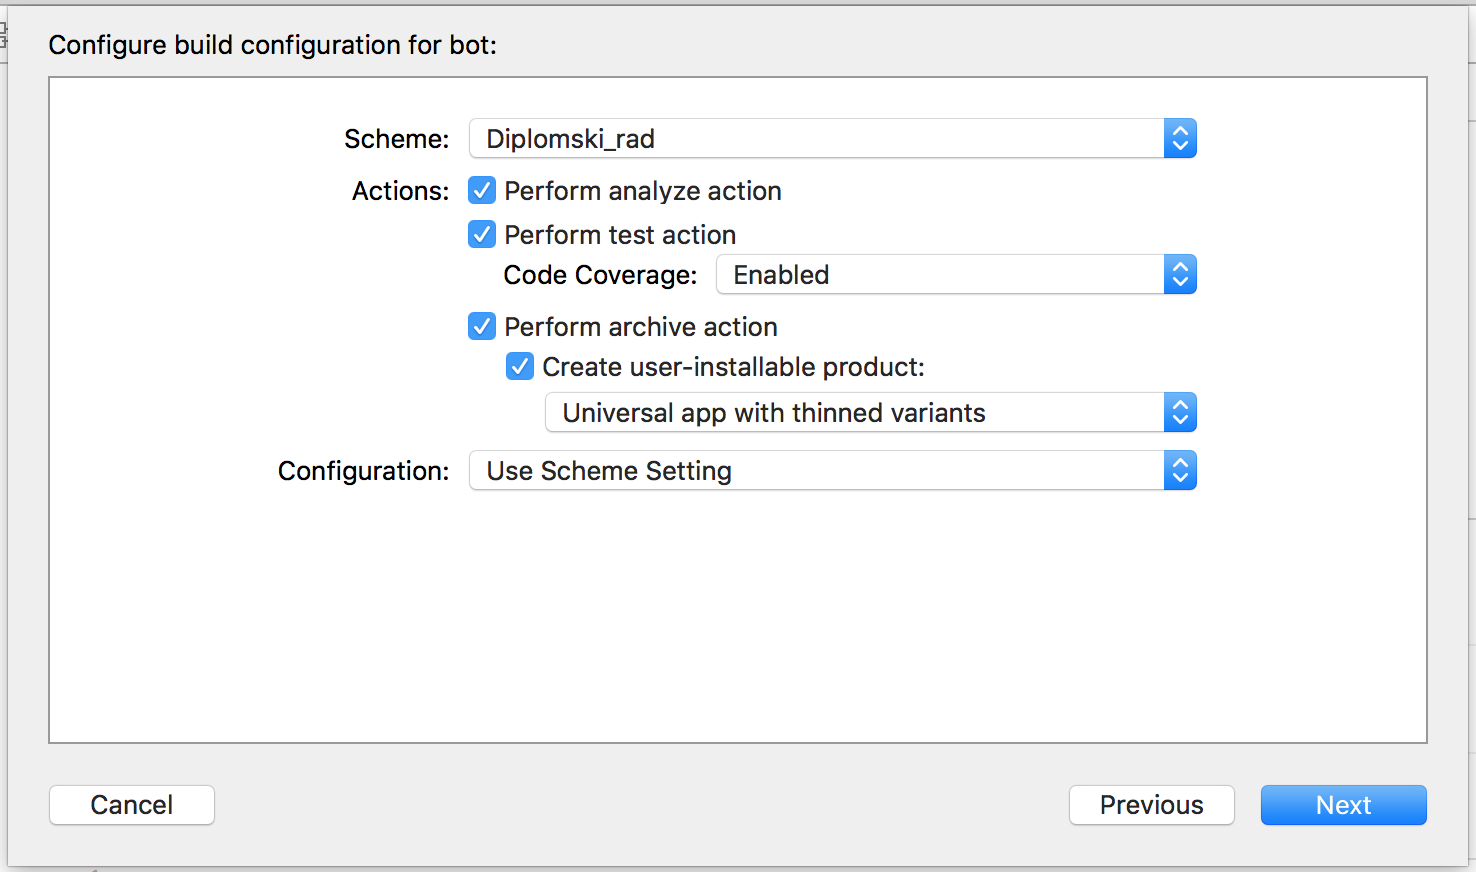
\includegraphics[scale=0.5]{XcodeServerOptions}
    \caption{Konfiguracija osnovnih opcija integracije}
    \label{fig:XcodeServerOptions}
\end{figure}

Moguće je postaviti kada se integracija izvršava. Opcije su periodički, nakon svakog spajanja ili ručno.

\begin{figure}
    \centering
    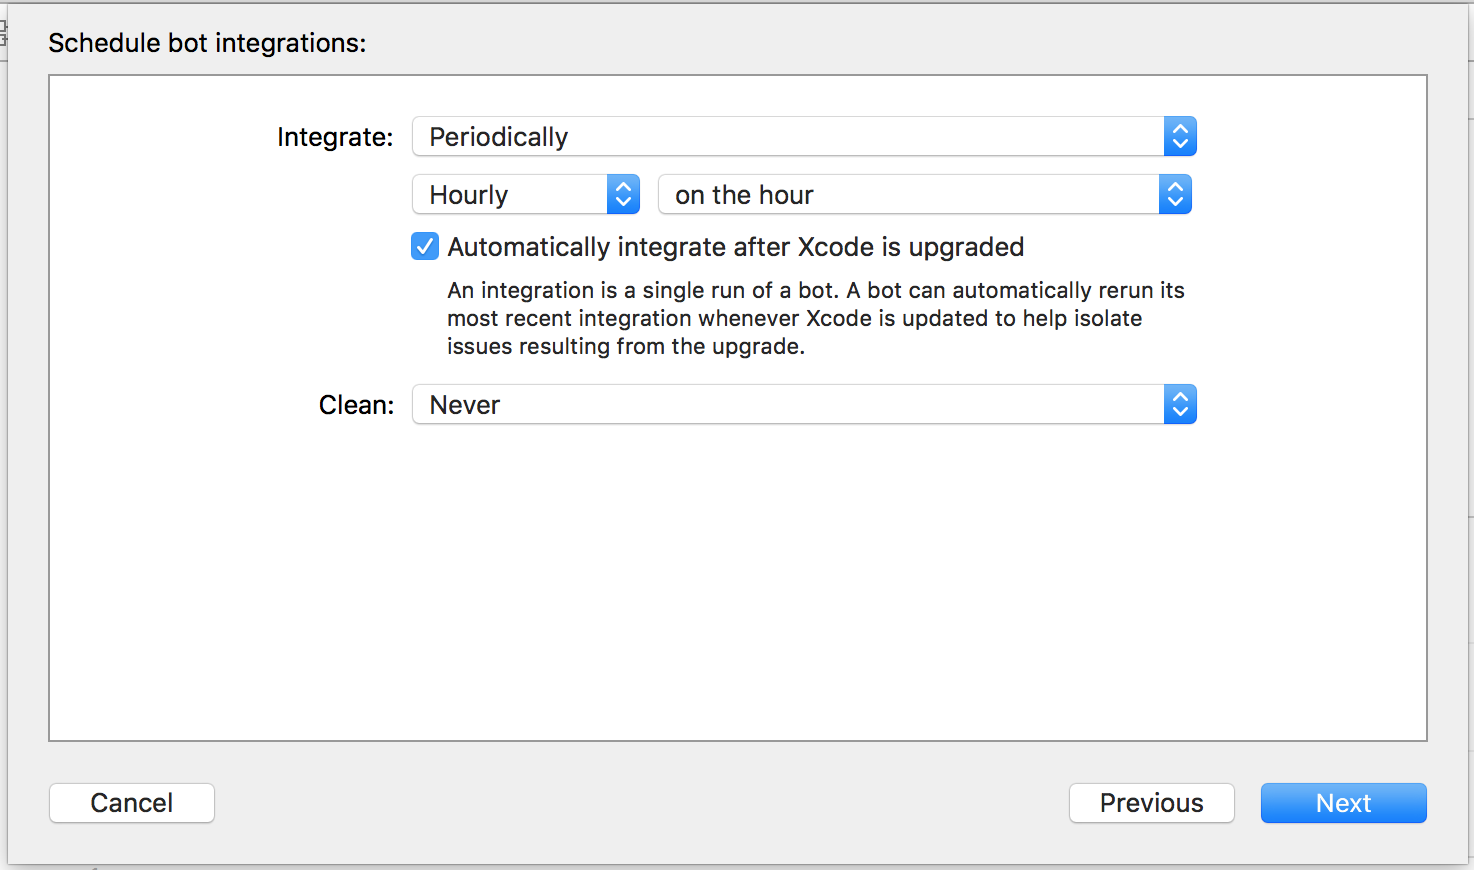
\includegraphics[scale=0.5]{XcodeServerIntegrationPeriods}
    \caption{Konfiguracija perioda izvršavanja integracije}
    \label{fig:XcodeServerIntegrationPeriods}
\end{figure}

Dodatno, moguće je konfigurirati okolinu u kojoj će se integracija izvršavati te akcije prije ili poslje obavljana integracije. Okolina se konfigurira pomoću kljuć - vrijednost parova. Akcije su proizvoljne skripte pokrenute u \textit{bin/sh} ljusci. Obje funkcionalnosti se ekstenzivno koriste za ostvarenje kontinuirane dostave i isporuke.

Ovime smo kreirali bot. Odmah nakon kreiranja bot započinje integraciju. Integraciju je moguće ručno započeti odabiron \textit{Integrate} opcije u gornjem desnom kutu.

Međutim, prva integracija ne prolazi. Problem izazivaju ovisnosti. Xcode Server preuzima sadržaj repozitorija izvornog te na njemu obavlja integraciju. Problem ovisnosti je moguće riješiti na dva naćina.

Sve potrebne ovisnosti je moguće dodati repozitoriju izvornog koda. Korištenjem navedenog postupka su sve ovisnosti prisutne u repozitoriju odmah nakon preuzimanja repozitorija zbog ćega ih nije potrebno dohvaćati. Navedeni postupak olakšava implementaciju i ubrzava proces integracije. Međutim, dodavenje svih ovisnosti u izvorni repozitorij nosi i značajne probleme. Prvo, repozitorij koda postaje znaćajno veći. Pregledom vlastitih projekata ustanovio sam da su ovisnosti od 2 do 50 puta veće od glavnog projekta. Ćak i u najvećem projektu su ovisnosti bile značajno veće od glavnog projekta. Navedeno povećanje repozitorija usporava preuzimanje i otežava praćenje promjena. Iako navedeni postupak ima svojih prednosti, generalno se izbjegava u praksi.

Drugi pristup je ovisnosti dohvatiti i pripremiti nakon dohvaćanja izvornog koda. Ovaj proces je vremenski vrlo zahtjevan. Dohvaćanje i ponovna izgradnja svih ovisnosti može značajno usporiti proces integracije. Zbog navedenog je vrlo važno dohvaćati samo potrebne ovisnosti. Ostvarivanje navedenog ponašanja značajno ovisi o alatu koji koristimo.

Implementacija prvog pristupa je vrlo jednostavna. Potrebno je sve ovisnosti dodati u repozitorij, odnosno maknuti ih \textit{.gitignore} dokumenta.

Implemnetacija drugog pristupa je nešto složenija. Snažno je preporučeno Xcode Server pokrenuti na zasebnom račun operacijskog sustava koji nema administrativna prava. Budući da se Xcode Serveru može pristupiti iz vanjske mreže važno je ograničiti prava koja navedeni alat posjeduje. Izdvajanjem procesa na zasebni račun osiguravamo da alat ima samo prava koja su mu potrebna. S druge strane, kompliciramo proces implementacije strogom kontrolom pristupa. Standardno je kreirati račun s imenom \textit{xcodeserver}.

Računu koji obavlja integraciju je potrebno dati potrebna prava te osigurati potrebne alate. Budući da želimo automatizirati što veću količinu posla, poželjno je sve potrebne alate instalirati u sklopu integracije, a ne zahtijevati njihovo postojanje na računalu. Međutim, što više funkcionalnosti nastojimo automatizirati to se implementacija integacije komplicira. Dodatno, neke alate ne možemo instalirati bez dopuštenja korisnika.

Za dohvat brojnih alata koristimo \textit{Homebrew} aplikacija. Međutim, instalacija navedene aplikacije zahtijeva \textit{sudo} lozinku. Dodatno, potrebno je xcodeserver računu dopustiti pristup \verb|/usr/local| direktoriju. Naredba pod (1) instalira Homberew, naredba pod (2) kreira ci grupu dok naredbe (3) i (4) omogućuju pristup xcodeserver računu.

\begin{verbatim}
#Homebrew
/usr/bin/ruby -e "$(curl -fsSL https://raw.githubusercontent.com
    /Homebrew/install/master/install)" (1)

sudo dseditgroup -o create ci (2)

sudo dseditgroup -o edit -a {current_user} -t user ci (3)
sudo dseditgroup -o edit -a xcodeserver -t user ci

sudo chgrp -R ci /usr/local (4)
sudo chmod -R g+wr /usr/local

\end{verbatim}

U integraciji koristim nekoliko alata napisanih u jeziku \textit{ruby}. Za njihovo lakše održavanje koristim alat \textit{RVM}. RVM olakšava instaliranje i upravljanje alatima napisanim u jeziku ruby.

RVM se predodređeno instalira na lokaciji \verb|~/.rvm/bin/rvm|. Prije pokretanja instalacija provjeravam postoji li rvm. U slučaju ne postojanja ga instaliram i konfiguriram.

\begin{verbatim}
if command -v ~/.rvm/bin/rvm >/dev/null 2>&1 ; then
    echo "RVM found"
else
    echo "RVM not found, proceeding with installation"

    \curl -sSL https://get.rvm.iwo | bash -s stable
    source ~/.rvm/scripts/rvm
fi
\end{verbatim}

Nakon instaliranje RVMa možemo instalirati CocoaPods alat. Za navedeno koristim sljedeću skriptu:

\begin{verbatim}
if command -v /usr/local/bin/podw >/dev/null 2>&1 ; then
    echo "CocoaPods found"
else
    echo "CocoaPods not found, proceeding with installation"

    /usr/local/bin/gem install cocoapods --user-install
    /usr/local/bin/pod setup
fi
\end{verbatim}

U slučaju ne postojanja CocoaPods alata, skripta ga instalira i konfigurira. Sada možemo iskoristiti alat za dohvat ovisnosti. Jednostavno se navigiramo u repozitorij i u slučaju postojanja Podfile datoteke dohvaćamo ovisnosti. Sljedeća naredba dohvaća verzije ovisnosti specificirane u \textit{Pofile.lock} datoteci. Ako ovisnost već postoji onda se ona ne dohvaća ponovno.

\begin{verbatim}
if [ -f Podfile ]; then
    pod install
fi
\end{verbatim}

Za instalaciju Carthage alata koristimo homebrew. Proces je sličan instalaciji CocoaPods alata.

\begin{verbatim}
if command -v /usr/local/bin/carthage >/dev/null 2>&1 ; then
    echo "Carthage found"
else
    echo "Carthage not found, proceeding with installation"

    if command -v /usr/local/bin/brew >/dev/null 2>&1 ; then
        echo "Homebrew needs to be installed "
    else
        brew install carthage
    fi
fi
\end{verbatim}

Dohvat ovisnosti je također sličan alatu CocoaPods.

\begin{verbatim}
if [ -f Cartfile ]; then
    echo "Fetching dependencies using Carthage"

    /usr/local/bin/carthage update --platform ios --cache-builds
else
    echo "Skipped fetching dependencies using Carthage"
fi
\end{verbatim}

Korištenjem opcije \verb|--cache-builds| spriječavamo izgradnu već postoječih ovisnosti.
















\end{appendices}

\end{document}
